\documentclass[a4paper,12pt]{article} % добавить leqno в [] для нумерации слева
\usepackage[a4paper,top=1.3cm,bottom=2cm,left=1.5cm,right=1.5cm,marginparwidth=0.75cm]{geometry}
%%% Работа с русским языком
\usepackage{cmap}					% поиск в PDF
\usepackage{mathtext} 				% русские буквы в фомулах
\usepackage[T2A]{fontenc}			% кодировка
\usepackage[utf8]{inputenc}			% кодировка исходного текста
\usepackage[english,russian]{babel}	% локализация и переносы
\usepackage{multirow}

\usepackage{graphicx}

\usepackage{wrapfig}
\usepackage{tabularx}

\usepackage{hyperref}
\usepackage[rgb]{xcolor}
\hypersetup{
colorlinks=true,urlcolor=blue
}

%%% Дополнительная работа с математикой
\usepackage{amsmath,amsfonts,amssymb,amsthm,mathtools} % AMS
\usepackage{icomma} % "Умная" запятая: $0,2$ --- число, $0, 2$ --- перечисление

%% Номера формул
\mathtoolsset{showonlyrefs=true} % Показывать номера только у тех формул, на которые есть \eqref{} в тексте.

%% Шрифты
\usepackage{euscript}	 % Шрифт Евклид
\usepackage{mathrsfs} % Красивый матшрифт

%% Свои команды
\DeclareMathOperator{\sgn}{\mathop{sgn}}

%% Перенос знаков в формулах (по Львовскому)
\newcommand*{\hm}[1]{#1\nobreak\discretionary{}
{\hbox{$\mathsurround=0pt #1$}}{}}

%% Графики
\usepackage{tikz}
\usepackage{pgfplots}
\pgfplotsset{compat=1.9}

\usepackage{subcaption}

\date{\today}

\begin{document}

\begin{titlepage}
	\begin{center}
		{\large МОСКОВСКИЙ ФИЗИКО-ТЕХНИЧЕСКИЙ ИНСТИТУТ (НАЦИОНАЛЬНЫЙ ИССЛЕДОВАТЕЛЬСКИЙ УНИВЕРСИТЕТ)}
	\end{center}
	\begin{center}
		{\large Физтех-школа прикладной математики и информатики}
	\end{center}
	
	
	\vspace{4.5cm}
	{\huge
		\begin{center}
			{\bf Отчёт о выполнении лабораторной работы 3.4.1}\\
			Диа- и парамагнетики
		\end{center}
	}
	\vspace{1cm}
	\begin{center}
		{\large Соболевский Федор Александрович \\
			\vspace{0.2cm}
			Б05-111}
	\end{center}
	\vspace{8cm}
	\begin{center}
		Ноябрь 2022
	\end{center}
\end{titlepage}

\section{Аннотация}

В данной работе были исследованы магнитные свойства диа- и парамагнетиков на примере образцов из различных металлов и графита. Были измерены значения магнитной восприимчивости материалов образцов. На основе измерений были сделаны выводы о магнитных свойстах диа- и парамагнетиков.

\section{Теоретические сведения}

\subsection{Определение магнитной восприимчивости} 

Магнитная восприимчивость тел может быть определена методом измерения сил, которые действуют на тела в магнитном поле. Существуют два классических метода таких измерений: метод Фарадея и метод Гюи. В методе Фарадея исследуемые образцы, имеющие форму маленьких шариков, помещаются в область сильно неоднородного магнитного поля и измеряется сила, действующая на образец. При этом для расчёта магнитной восприимчивости необходимо знать величину градиента магнитного поля в месте расположения образца. В методе Гюи используется тонкий и длинный стержень, один из концов которого помещают в зазор электромагнита (обычно в область однородного поля), а другой конец~-- вне зазора, где величиной магнитного поля можно пренебречь. Закон изменения поля~-- от максимального до нулевого -- в этом случае несуществен.

Найдём выражение для магнитной силы, действующей на такой образец (рис. \ref{pic:2}). Пусть площадь образца равна $ s $, его магнитная проницаемость~-- $ \mu $, а поле в зазоре равно $ B $.

\begin{figure}[h]
\centering
    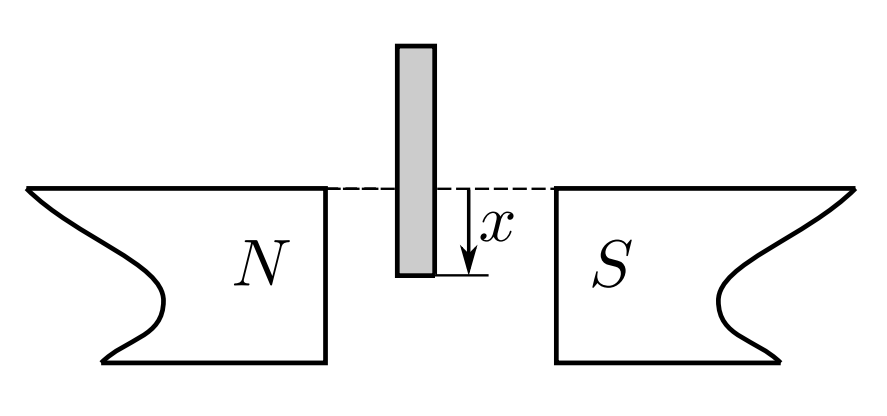
\includegraphics[width=0.5\textwidth]{2.png}
    \caption{Расположение образца в зазоре электромагнита}
    \label{pic:2}
\end{figure}

Воспользуемся для расчёта энергетическими соображениями. Магнитная сила может быть вычислена как производная от магнитной энергии по перемещению. Данную производную следует брать со знаком минус, когда образец находится в поле постоянного магнита, или со знаком плюс, как в нашем случае, когда поле в зазоре создаётся электромагнитом, ток $ I $ в обмотках которого поддерживается постоянным.

При смещении образца на расстояние $ \Delta l $ вниз магнитная сила, действующая на него, равна

\begin{equation}\label{1}
F = \left(\frac{\Delta W_m}{\Delta l}\right)_I,
\end{equation}
где $ \Delta W_m $ -- изменение магнитной энергии системы при постоянном токе
в обмотке электромагнита и, следовательно, при постоянной величине
магнитного поля в зазоре.

Магнитная энергия рассчитывается по формуле

\begin{equation}\label{2}
W_m=\frac{1}{2}\int HBd\,V = \frac{1}{2\mu_0}\int\frac{B^2}{\mu}d\,V,
\end{equation}
где интеграл распространён на всё пространство. При смещении образца магнитная энергия меняется только в области зазора (в объёме площади $ s $ и высоты $ \Delta l $), а около верхнего конца стержня остаётся неизменной, поскольку магнитного поля там практически нет. Принимая поле внутри стержня равным измеренному нами полю в зазоре $ B $, получим

\begin{equation}\label{3}
\Delta W_m=\frac{1}{2\mu_0}\frac{B^2}{\mu}s\Delta l - \frac{1}{2\mu_0}B^2 s\Delta l = -\frac{\chi}{2\mu_0\mu}B^2s\Delta l.
\end{equation}

Следовательно, на образец действует сила

\begin{equation}\label{4}
F = -\frac{\chi}{2\mu_0\mu}B^2s.
\end{equation}

Знак силы, действующей на образец, зависит от знака $ \chi $: образцы из парамагнитных материалов $( \chi > 0)$ втягиваются в зазор электромагнита, а диамагнитные образцы $ (\chi < 0) $ выталкиваются из него.

Пренебрегая отличием $ \mu $ от единицы, получаем окончательно расчётную формулу в виде

\begin{equation}\label{5}
F = -\frac{\chi B^2s}{2\mu_0}.
\end{equation}

Измерив силу, действующую на образец в магнитном поле $ B $, можно рассчитать магнитную восприимчивость образца.

\subsection{Экспериментальная установка}

\begin{figure}[h]
    \centering
    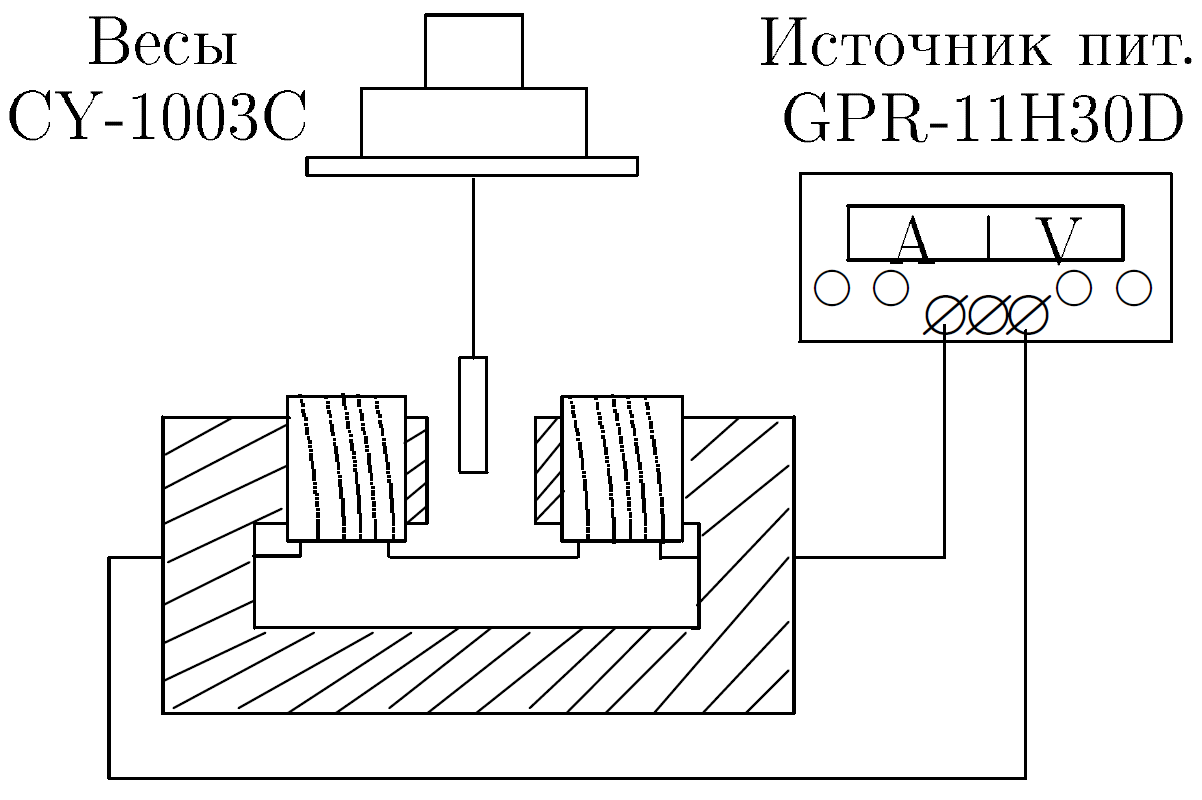
\includegraphics[width=0.6\textwidth]{1.png}
    \caption{Схема экспериментальной установки.}
    \label{pic:1}
\end{figure}

Магнитное поле с максимальной индукцией $ \simeq 1 $ Тл создаётся в зазоре электромагнита, питаемого постоянным током. Диаметр полюсов существенно превосходит ширину зазора, поэтому поле в средней части зазора достаточно однородно. Величина тока, проходящего через обмотки электромагнита, задаётся регулируемым источником питания GPR и измеряется амперметром $A$, встроенным в источник питания. Градуировка электромагнита (связь между индукцией магнитного поля $B$ в зазоре электромагнита и силой тока $ I $ в его обмотках) производится при помощи милливеберметра.

При измерениях образцы поочерёдно подвешиваются к весам так, что один конец образца оказывается в зазоре электромагнита, а другой -- вне зазора, где индукцией магнитного поля можно пренебречь. При помощи весов определяется перегрузка $ \Delta P = F $ -- сила, действующая на образец со стороны магнитного поля.


Силы, действующие на диа- и парамагнитные образцы, очень малы. Небольшие примеси ферромагнетиков (сотые доли процента железа или никеля) способны кардинально изменить результат опыта, поэтому образцы были специально отобраны.

\section{Оборудование и инструментальные погрешности}

\textbf{В работе использовались:} электромагнит, аналитические весы, миллибеберметр, магнитометр, регулируемый источник постоянного тока, образцы из меди, вольфрама, алюминия.

\textbf{Инструментальные погрешности:}
\begin{itemize}
    \item \textbf{Амперметр:} $\Delta_I = 0,01$ А;
    \item \textbf{Милливеберметр:} $\Delta_{B_1} = 0,1$ мВб;
    \item \textbf{Магнитометр:} $\Delta_{B} = 5$ Тл;
    \item \textbf{Весы:} $\Delta_m = 0,5$ мг.
\end{itemize}

В работе для измерения индукции магнитного поля использован магнитометр, так как милливеберметр даёт большую, чем у магнитометра, относительную погрешность измерений. 

\section{Результаты измерений и обработка экспериментальных данных}

\subsection{Градуировка электромагнита}

Перед проведением опыта была проведена градуировка магнита. С помощью магнитометра было измерено значение магнитной индукции между полюсами электромагнита в зависимости от тока с шагом в $ 0,5 $ А. Результаты измерений представлены в таблице \ref{tab:my-table1}.

\begin{table}[h]
    \centering
    \begin{tabular}{|c|c|c|c|c|c|c|}
	\hline
	$ I $, А  & 0,5  & 1,0  & 1,5  & 2,0  & 2,5  & 3,0  \\ \hline
	$ B $, Гс & 1755 & 3181 & 4696 & 6106 & 7309 & 8291 \\ \hline
    \end{tabular}
    \caption{Зависимость индукции магнитного поля катушки от силы тока в ней}
    \label{tab:my-table1}
\end{table}

\subsection{Измерение сил, действующих на образцы в магнитном поле}

Для четырех образцов из меди, вольфрама, алюминия и графита соответственно были измерены силы $F$, действующей на образец при различных токах в обмотках электромагнита. Величина данной силы определялась как разность $\Delta P$ между весом груза при отключенном электромагните и при данном токе через него. Результаты измерений представлены в таблице \ref{tab:my-table2}. Зависимость величины силы от индукции магнитного поля представлена на рис. 3 и 4.

\begin{table}[h]
\begin{center}
   \begin{tabular}{|c|c|c|c|c|c|} \hline
    $I$, А & $B$, Гс & $\Delta P_\text{Cu}/g$, мг & $\Delta P_\text{W}/g$, мг & $\Delta P_\text{Al}/g$, мг & $\Delta P_\text{C}/g$, мг \\ \hline 
    0,5 & 1755 &  -1 &  0 &  2 &  -33 \\ \hline 
    1,0 & 3181 &  -3 &  2 &  6 &  -80 \\ \hline
    1,5 & 4696 &  -7 &  4 & 14 & -133 \\ \hline
    2,0 & 6106 & -11 &  8 & 24 & -186 \\ \hline
    2,5 & 7309 & -17 & 12 & 35 & -268 \\ \hline
    3,0 & 8291 & -22 & 17 & 46 & -315 \\ \hline
    \end{tabular} 
\end{center}    
\caption{Результаты измерений сил, действующих на образцы в магнитном поле}
\label{tab:my-table2}
\end{table}

По графику зависимости отклоняющей силы для графита видно, что погрешность её измерения очень велика. Это связано с тем, что при включении достаточно сильного поля образец притягивался к одной из стенок зазора в электромагните, и весы фиксировали неточные значения вследствие наличия трения между образцом и стенкой.

\begin{figure} \label{graph1}
\begin{center}
\begin{tikzpicture}
    \begin{axis}[
    xlabel={$B^2$, Тл$^2$},
    ylabel={$|\Delta P|$, мН},
    legend pos=north west,
    xmajorgrids=true,
    ymajorgrids=true,
    grid style=dashed,
    width = 400,
    height = 280,
    xmin = 0,
    ymin = 0,
    xmax = 1,
    ymax = 5
    ]
    \addplot[color=black, mark=x, mark size = 4pt, only marks] coordinates{
    (0.031, 0.102)
    (0.101, 0.306)
    (0.221, 0.714)
    (0.373, 1.121)
    (0.534, 1.733)
    (0.687, 2.243)
    };
    \addplot[color=black, mark=o, mark size = 5pt, only marks] coordinates{
    (0.031, 0)
    (0.101, 0.204)
    (0.221, 0.408)
    (0.373, 0.815)
    (0.534, 1.223)
    (0.687, 1.733)
    };
    \addplot[color=black, mark=triangle, mark size = 4pt, only marks] coordinates{
    (0.031, 0.204)
    (0.101, 0.612)
    (0.221, 1.427)
    (0.373, 2.446)
    (0.534, 3.568)
    (0.687, 4.689)
    }; 
    \legend{Медь, Вольфрам, Алюминий}
    \addplot[color=blue]{3.215*x};
    \addplot[color=purple]{2.361*x};
    \addplot[color=red]{6.715*x};
    \end{axis}
\end{tikzpicture}
\caption{Графики зависимостей сил, действующих на металлические образцы, от величины поля}
\end{center}
\end{figure}

\begin{figure} \label{graph2}
\begin{center}
\begin{tikzpicture}
    \begin{axis}[
    xlabel={$B^2$, Тл$^2$},
    ylabel={$|\Delta P|$, мН},
    legend pos=north west,
    xmajorgrids=true,
    ymajorgrids=true,
    grid style=dashed,
    width = 300,
    height = 280,
    xmin = 0,
    ymin = 0,
    xmax = 0.75,
    ymax = 35
    ]
    \addplot[color=black, mark=x, mark size = 16pt, only marks] coordinates{
    (0.031, 3.364)
    (0.101, 8.155)
    (0.221, 13.558)
    (0.373, 18.96)
    (0.534, 27.319)
    (0.687, 32.11)
    };
    \legend{Графит}
    \addplot[color=blue]{49.809*x};
    \end{axis}
\end{tikzpicture}
\caption{Графики зависимости силы, действующей на образец из графита, от величины поля}
\end{center}
\end{figure}

Значения коэффициентов наклона $k = d(\Delta P)/d(B^2)$ следующие:

\begin{itemize}
    \item \textbf{Медь:} $k_\text{Cu} = -3,2 \pm 0,3$ мН/Тл$^2$;
    \item \textbf{Вольфрам:} $k_\text{W} = 2,4 \pm 0,3$ мН/Тл$^2$;
    \item \textbf{Алюминий:} $k_\text{Al} = 6,7 \pm 0,4$ мН/Тл$^2$;
    \item \textbf{Графит:} $k_\text{C} = -49,8 \pm 4,8$ мН/Тл$^2$.
\end{itemize}

\subsection{Расчёт величины магнитной восприимчивости}

Согласно формуле \eqref{5}, вычислим коэффициент магнитной восприимчивости $\chi$ для каждого образца. Из этой формулы следует, что

\begin{equation}\label{6}
    k = \frac{\chi s}{2\mu_0}.
\end{equation}

Отсюда

\begin{equation}\label{7}
    \chi = \frac{2\mu_0 k}{s}
\end{equation}

где $ s $~-- площадь поперечного сечения исследуемых образцов. В нашем случае $ s = (0,78 \pm 0,02) $ см$^2 $ для всех образцов. Получены следующие значения магнитной восприимчивости:

\begin{itemize}
    \item \textbf{Медь:} $\chi_\text{Cu} = -(1,03 \pm 0,08)\cdot 10^{-5}$;
    \item \textbf{Вольфрам:} $\chi_\text{W} = (0,76 \pm 0,06)\cdot 10^{-5}$;
    \item \textbf{Алюминий:} $\chi_\text{Al} = (2,16 \pm 0,18)\cdot 10^{-5}$;
    \item \textbf{Графит:} $\chi_\text{C} = -(16,0 \pm 1,5)\cdot 10^{-5}$.
\end{itemize}

\section{Обсуждение результатов и выводы}

В ходе данной работы была измерена магнитная восприимчивость диа- и пара- магнетиков. Были исследованы образцы из меди, вольфрама, алюминия и графита. Табличные значения измеренных величин представлены в таблице \ref{tabres}. Полученные экспериментально значения для металлов совпадают с табличными в пределах погрешностей. Исходя из результатов эксперимента можно сказать, что алюминий и вольфрам являются парамагнетиками $ (\chi > 0) $, а медь в свою очередь~-- диамагнетиком $ (\chi < 0) $. Значение для графита также близко к табличному, однако относительная погрешность определения магнитной восприимчивости в данном случае выше, чем для остальных образцов. Исходя из эксперимента, графит также является диамагнетиком.

\begin{table}[h!]
\begin{center}
\begin{tabular}{|c|c|c|c|c|}
\hline
Материал & Медь & Вольфрам & Алюминий & Графит \\ \hline
Измеренное значение, $10^{-5}$ & $-1,03\pm 0,08$ & $0,76\pm 0,06$ & $2,16 \pm 0,18$ & $-16,0 \pm 1,5$ \\ \hline
Табличное значение, $10^{-5}$ & -0,96 & 0,64 & 2,2 & -14 \\ \hline
\end{tabular}
\end{center}
\caption{Измеренные и теоретические значения магнитной восприимчивости}
\label{tabres}
\end{table}

Таким образом, описанный выше метод измерения магнитной проницаемости материалов является рабочим и позволяет с хорошей точность определить эту величину для различных исследуемых образцов. Использованная экспериментальная установка обеспечивает высокую точность при измерении магнитной восприимчивости металлов; для повышения точности измерений для графита следует сделать зазор между обкладками электромагнита больше либо взять меньший по толщине или больший по массе образец графита.

\end{document}